\apendice{Plan de Proyecto Software}

\section{Introducción}

En el apartado aquí descrito se comenta cómo ha sido el seguimiento de este  proyecto. La metodología utilizada es Scrum que se emplea en los proyectos ágiles y que consiste en un desarrollo colaborativo en el que se hacen entregas periódicas de las diferentes partes del proyecto hasta juntar un todo que forme el proyecto final. 

Para ello hemos hecho uso de herramientas como GitHub y ZenHub que ayudan en la labor de definir objetivos semanales o Milestones que a su vez están compuestos por problemas denominados issues. También hemos podido ver el progreso semanal, comunicar aspectos relacionados con el trabajo o agrupar los issues según el tipo.

Como en cualquier proyecto de este tipo, a veces, algunos objetivos semanales se han modificado debido a que resultaban más complejos de lo esperado o inútiles para el fin buscado o no accesibles como es el caso, por ejemplo, de los elementos para el desarrollo de interfaces con Vaadin, que requerían una licencia de pago muy elevada. Todo ello forma parte de la gestión de proyectos ágiles.

\section{Planificación temporal}

El desarrollo del proyecto esta compuesto por entregas periódicas denominadas sprints y que han tenido una duración de una semana, a excepción del sprint número nueve que por motivos de vacaciones escolares tuvo que ser del doble de tiempo. Aunque al principio el seguimiento del proyecto no fue el correcto en cuanto al manejo de las herramientas GitHub  y ZenHub, posteriormente se trató de mejorarlo.

Se trató de llevar una carga constante de trabajo para mantener un ritmo con el que se llegase a la fecha de entrega, pero en alguno de los últimos sprints se tuvo que aumentar la cantidad porque había más materia sobre la que trabajar y mejorar.

En total fueron unas 21 semanas en las que se simulan los sprints mediante milestones con objetivos definidos en las reuniones entre tutores y alumno, desde el mes de febrero hasta junio. Cada issue va dentro de milestone determinado, especificando el tipo de issue y el tiempo estimado hasta su resolución. Se hace uso de Git como gestor de versiones. 

\subsection{Sprint 0 (1/2/2017 - 8/2/2017)}

En este primer <<Sprint>> determinamos que posibles herramientas de traducción pueden ser útiles para este proyecto sin profundizar demasiado. Se hace también la primera toma de contacto con Thoth para ver su funcionamiento básico.

Por otro lado, analizamos las posibilidades del proyecto, determinando los caminos en los que puede derivar dicho proyecto. Es decir, en estos primeros pasos no sabemos como funcionan estas herramientas, es por ello que el resultado sea más simple del esperado o por el contrario resulten complicaciones que lleven un tiempo mayor al esperado.

Además de esto, hacemos una introducción a las herramientas de documentación y gestión. Por ello aclaramos que:

\begin{itemize}
\item Para la gestión de versiones haremos uso de GitHub, asociando un gestor de tareas llamado Zenhub que funciona como un <<plugin>> en el buscador.
\item Realizo un primer contacto con \LaTeX 
\end{itemize}

En esta primeras semanas no me aclaro mucho con el funcionamiento del gestor de versiones, y es por ello que no hago un buen uso de los <<commits>> ni de los <<issues>> que proporciona Github.

\subsection{Sprint 1 (8/2/2017 - 15/2/2017)}

Ya en la segunda semana realizo una evaluación más exhaustiva de las herramientas de traducción, analizando los pros y los contras de ellas. Por lo tanto tomamos la decisión de centrarnos en GWT como la principal y con la que vamos a llevar a cabo el proyecto.

Definimos como tareas semanales:

\begin{itemize}
\item Evaluar los pros y contras de las diferentes herramientas de traducción de código.
\item Documentar esa evaluación con \LaTeX , familiarizándome con la manera de documentar.
\item Realizar las primeras pruebas con GWT, de una forma simple.
\end{itemize}

En esta semana hago alguna prueba simple con GWT, gracias a los ejemplos que proporciona la página oficial a modo de tutorial. También realizo alguna prueba simple con JSweet para ver su funcionamiento real y si es, de verdad, útil para poder llevar a cabo el proyecto. En el último ejemplo que hago me ocurre un problema con GWT que no termino de solucionar y que me obliga a posponer la prueba de ese ejemplo para el siguiente sprint.

También profundizo algo más en la documentación y en el uso de las herramientas para documentar. Hasta este punto no he asociado las tareas o <<issues>> con los <<milestones>> y por lo tanto no queda registrado el tiempo del sprint.

\subsection{Sprint 2 (15/2/2017 - 22/2/2017)}

En este tercer sprint, lo primero que hago es solucionar el anterior problema que tuve con GWT. Consistía en configurar bien el entorno de Eclipse y el <<plugin>> para poder hacer la ejecución de GWT con <<Super Dev Mode>>, alternativa implantada por los desarrolladores para evitar la necesidad de instalar una extension de GWT en el buscador en el cual se lanza la aplicación. El burdown chart del sprint 2 se ilustra en la figura \ref{fig:A.1}.

\begin{figure}[h]
\centering
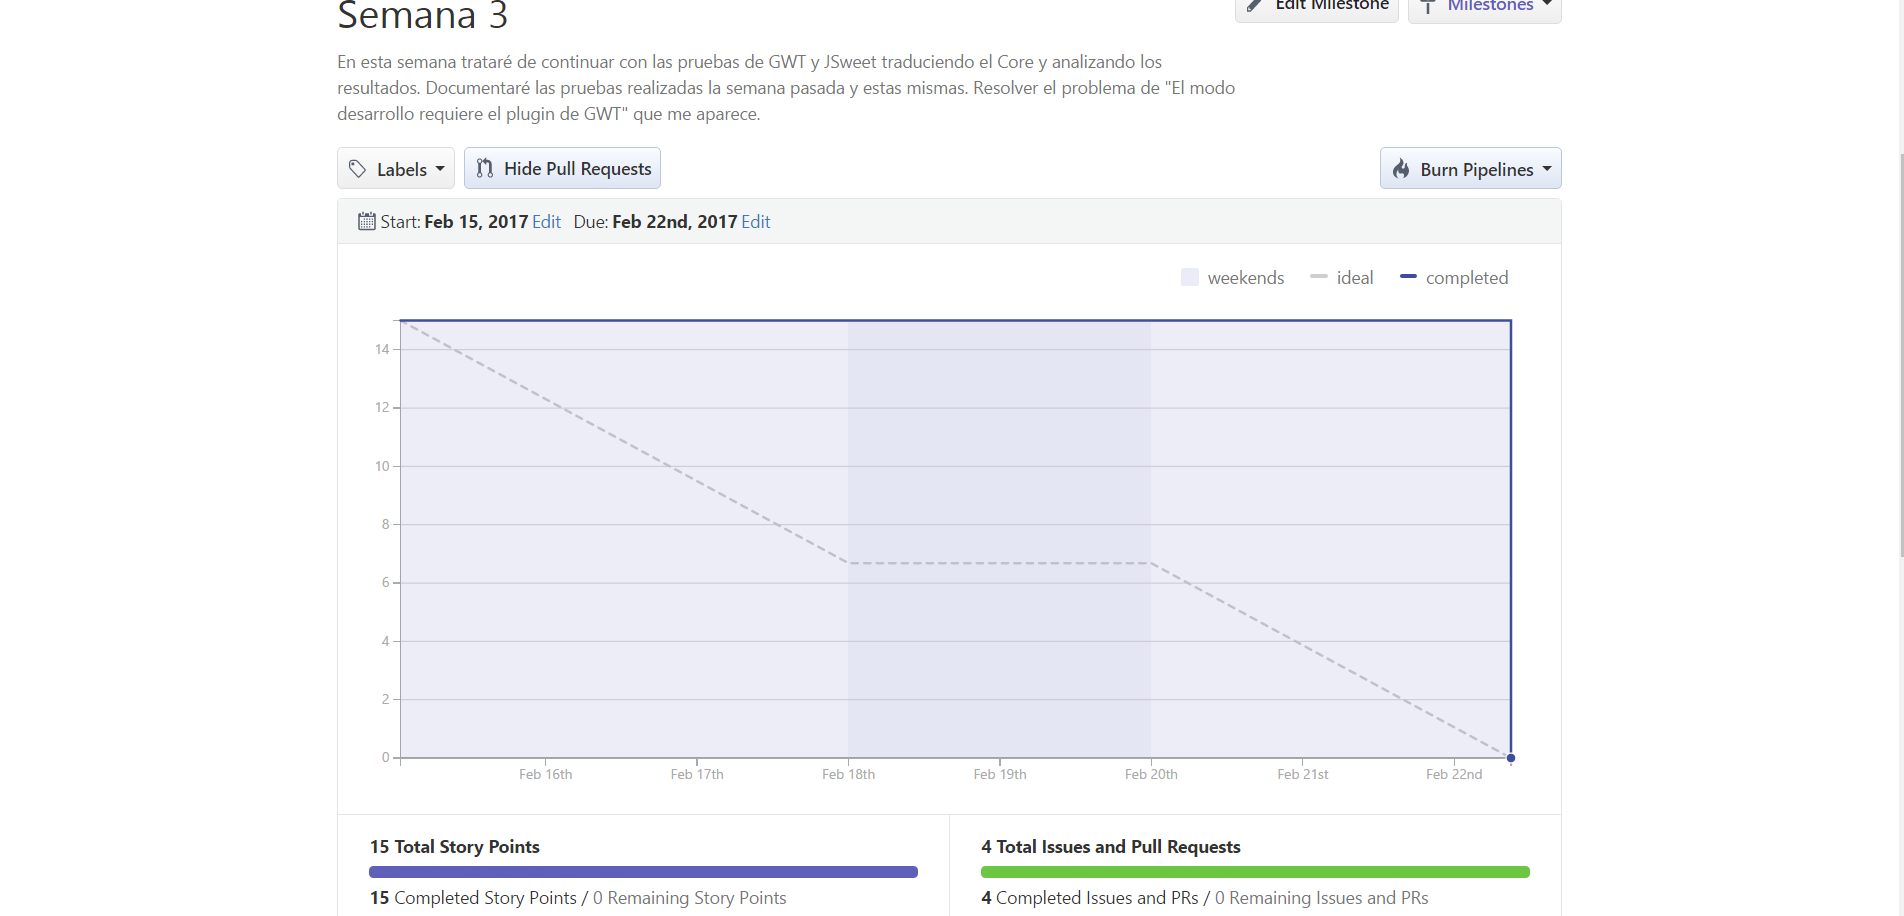
\includegraphics[width=0.99\textwidth]{Semana3}
\caption{Burndown del sprint 2}
\label{fig:A.1}
\end{figure}

También en esta semana descubrimos una nueva herramienta relacionada con el tema, que se llama Vaadin y que nos puede servir, por lo menos para hacer una comparativa más completa de las herramientas de traducción. 

La parte más importante de esta semana es la prueba de traducción del <<core>> de Thoth, que aunque no sale como esperamos, ha resultado útil para conocer con mayor profundidad tanto la aplicación como la herramienta.

Por lo tanto como tareas para este sprint:

\begin{itemize}
\item Solucionar el error surgido con GWT.
\item Realizar pruebas de traducción con el <<core>> de Thoth.
\item Incluir la nueva herramienta en la comparativa.
\end{itemize}

Muy a mi pesar, en el <<milestone>> de esta semana, aunque he pasado cada tarea al estado de realizada o <<done>> no las he cerrado hasta darnos cuenta al final del sprint, es por ello que el <<burndown>> queda de esta manera.


\subsection{Sprint 3 (22/2/2017 - 1/3/2017)}

Ya en la cuarta semana se hace un intento más completo para traducir la aplicación. Como pudimos comprobar en la semana pasada, GWT no traducía las librerías de la parte visual de Thoth. Es por ello decidimos hacer un ejemplo de forma manual que consiste en programar parte de la vista que esta asociada a las partes más relevantes del núcleo.

Por ejemplo, nos centramos en hacer una prueba con la gramática, que esta dentro del núcleo, creando una pantalla con un <<text label>> para comprobar si funcionaba la traducción de esa parte del núcleo. De esta forma podríamos ver como hacía la traducción de todo el núcleo, ya que las otras partes de las que se compone son similares en el uso de librerías y bibliotecas.

Quedan así asignadas las tareas para del sprint número tres:

\begin{itemize}
\item Transformar la Gramática del núcleo de Thoth.
\item Transformar el Autómata del núcleo.
\item Transformar la simulación del núcleo de Thoth.
\item Documentar toda esta parte.
\end{itemize}

Al final solo se pudo llevar a cabo la tareas de la Gramática y la documentación porque no se pudo avanzar a las otras como muestra la imagen \ref{fig:A.2}.

\begin{figure}[h]
\centering
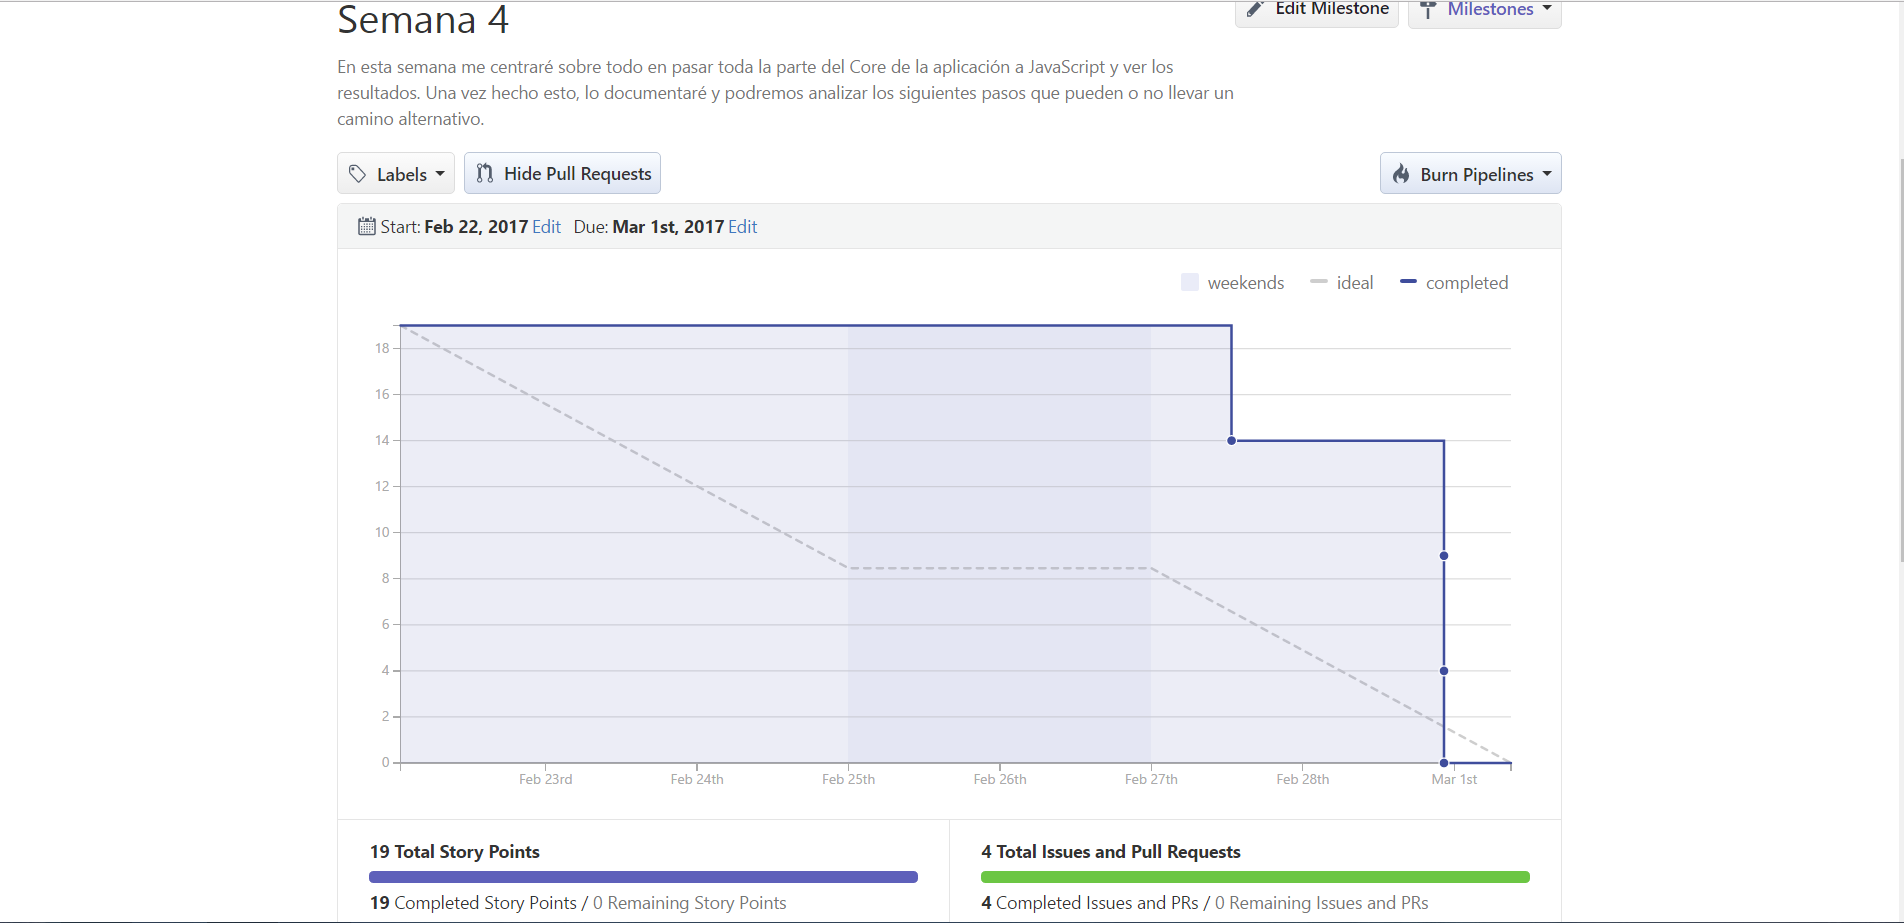
\includegraphics[width=0.99\textwidth]{Semana4}
\caption{Burndown del sprint 3}
\label{fig:A.2}
\end{figure}

 Nuestra idea era probar a tratar de traducir todo, núcleo incluido, ejecutando esas partes en el cliente de GWT  pero vimos que esto no es posible. Intentamos hacerlo de varias formas eliminando partes no esenciales de la aplicación para reducir errores de compilación hasta darnos por vencidos y ver que esa no era la solución.

\subsection{Sprint 4 (1/3/2017 - 8/3/2017)}
Hemos intentado pasar la aplicación en la parte del servidor y probar por nuestra cuenta. Sólo hemos metido el núcleo en el paquete servidor para ver que surgía. Como vimos que no había una comunicación entre el cliente y el servidor hicimos varios intentos, probando con el paquete de <<shared>> o compartido, pero GWT también traduce ese paquete a JavaScript por lo que seguía dando los mismo errores que en el cliente.

Por lo tanto en este sprint tenemos esta tareas:

\begin{itemize}
\item Solucionar un error en la traducción.
\item Realizar pruebas cliente-servidor con el núcleo de la aplicación.
\item Cambios y mejoras en la documentación.
\end{itemize}

Una vez nos dimos cuenta de que el fallo de tratar de hacer la aplicación en la parte del servidor era que GWT no reconocía algunas de las librerías claves, tanto en la parte visual como en el núcleo de la aplicación, decidimos buscar otros caminos alternativos. 


\begin{figure}[h]
\centering
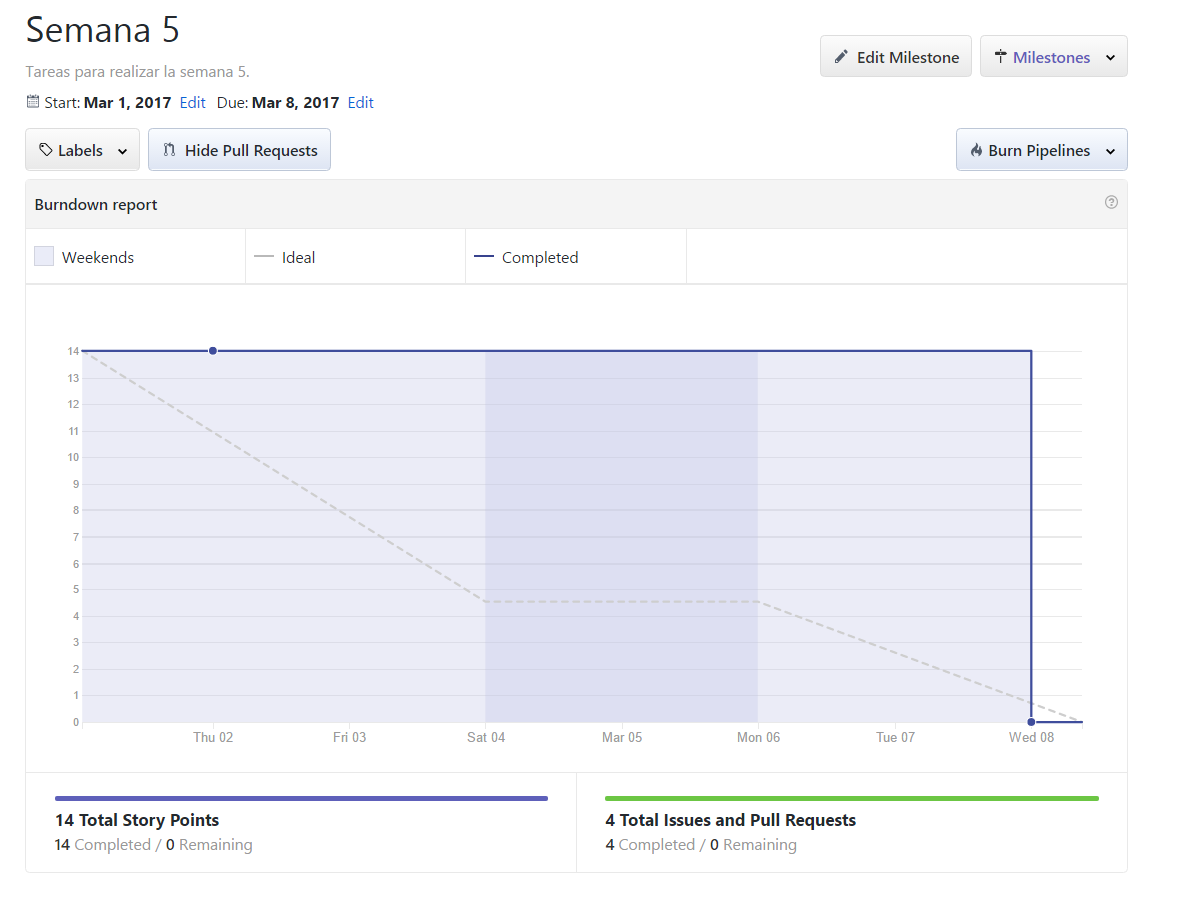
\includegraphics[width=0.99\textwidth]{Semana5}
\caption{Burndown del sprint 4}
\label{fig:A.3}
\end{figure}

El funcionamiento de GWT consiste en traducir a <<JavaScript>> la parte del cliente y la compartida. En consecuencia decidimos hacer pruebas en las que las partes mas fundamentales del núcleo se encontrasen en el lado del servidor. De esta forma cuando el cliente necesitase hacer algún uso de métodos con librerías no reconocidas por GWT, simplemente llamase al servidor ya que este podría soportar dichos métodos. 

En los primeros intentos nos dimos cuenta de que estas llamadas no se podían hacer de una forma simple, ya que la comunicación entre cliente y servidor no funcionaba y no obteníamos los resultados que esperábamos. Aún así seguimos haciendo pruebas para asegurarnos, metiendo dentro del paquete <<compartido>> las partes del núcleo mas cercanas a lo que nosotros consideramos la vista. El problema seguía siendo esa comunicación. Interpretaba como del lado del cliente lo que nosotros queríamos que formara parte del servidor, dando errores debido a que GWT no trabaja con esas librerías.

\subsection{Sprint 5 (8/3/2017 - 15/3/2017)}

Principalmente, en este quinto sprint, se llevan a cabo las pruebas para entender y poder evaluar la comunicación cliente-servidor, por medio de unos ejemplos. Además de eso, planteamos la idea de realizar un <<login>> y validación de usuarios, pero solo como idea, ya que no es prioritario al cien por cien importancia.

\begin{figure}[h]
\centering
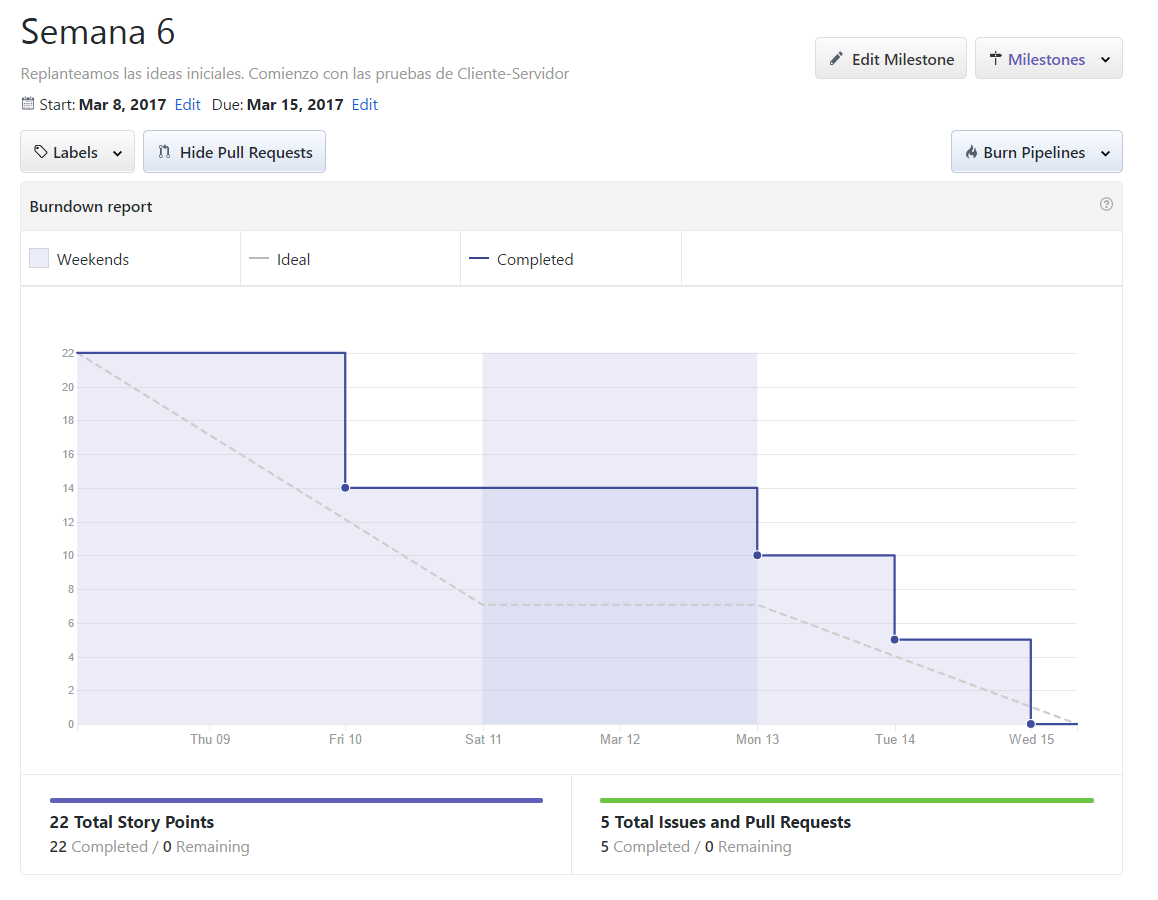
\includegraphics[width=0.99\textwidth]{Semana6}
\caption{Burndown del sprint 5}
\label{fig:A.4}
\end{figure}


Así que en este sprint tenemos esta tareas:

\begin{itemize}
\item Ejemplo cliente-servidor con GWT.
\item Login y validación en GWT.
\end{itemize}

Como se puede ver en el burdown chart del sprint 5  en la figura \ref{fig:A.4}, se trabajó de forma continuada en esta semana.
La comunicación entre el cliente y el servidor se lleva a cabo mediante la comunicación RPC (Remote Procedure Call). Es por ello que se hace necesario entender y practicar el funcionamiento de esta práctica. Los ejemplos realizados han sido dos: el primero es un ejemplo o tutorial ofrecido por la página oficial de GWT, que consiste en hacer un visor del <<stock>> que cambia de forma aleatoria sus valores. Y el segundo ejemplo consistió en hacer un pequeño ejemplo de llamada de funciones con más clases que en el anterior.


\subsection{Sprint 6 (15/3/2017 - 22/3/2017)}

En esta semana nos metemos ya en serio con la aplicación propiamente dicha. Lo primero que hacemos es conseguir que la comunicación entre en núcleo (ya hecho) y su uso sea fluido. Para ello lo que hacemos es incluir algunas partes en el cliente y otras en el servidor. En el cliente sólo podemos incluir las clases más simples, más primitivas de la aplicación porque su contenido es entendido por GWT y puede hacer la traducción a JavaScript sin problemas de librerías.

\begin{figure}[h]
\centering
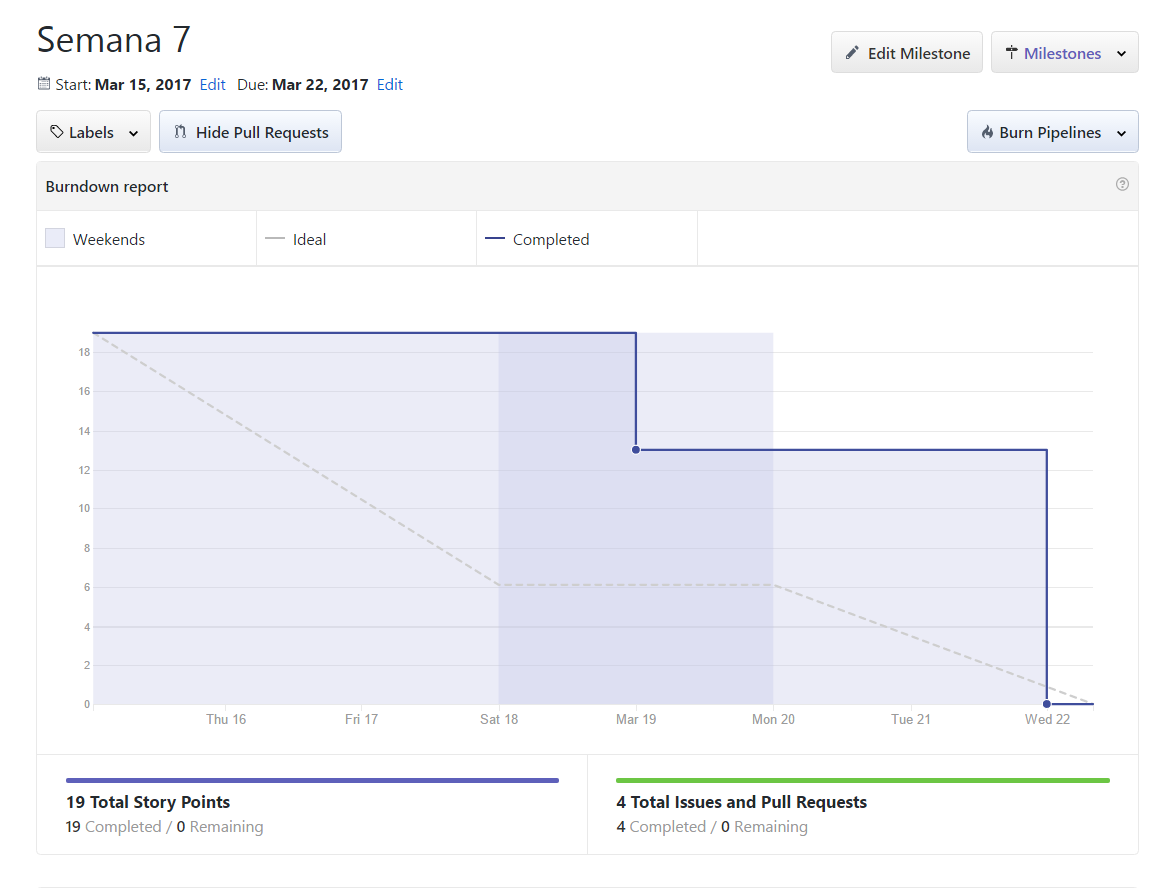
\includegraphics[width=0.99\textwidth]{Semana7}
\caption{Burndown del sprint 6}
\label{fig:A.5}
\end{figure}

Por lo tanto las tareas son básicamente dos:

\begin{itemize}
\item Llevar a cabo el primer prototipo o sección de la aplicación.
\item Documentar y corregir errores anteriores en la documentación.
\end{itemize}

La realización del prototipo nos lleva tiempo ya que se necesita comprender muy bien el funcionamiento interno de Thoth y así poder definir un diseño del software adecuado según ese funcionamiento. Una vez hecho eso parece simplificarse los problemas que al principio se tenían. Puede verse el burdown chart de este sprint en la figura\ref{fig:A.5}.

\subsection{Sprint 7 (22/3/2017 - 29/3/2017)}

Parece ser que en esta octava semana ya podemos empezar a trabajar más en la programación del diseño e implementar funcionalidades. Lo primero que tenemos que hacer es que esa comunicación entre métodos de resultados <<más>> visibles e integrarlos en una <<GUI>> denominada en español como interfaz gráfica de usuario. Para más detalles sobre la semana, ver la figura\ref{fig:A.6}

Así es que definimos como tareas las siguientes:

\begin{itemize}
\item Reestructurar la aplicación y limpiar el código.
\item Mejorar la GUI con Vaadin, ya que la anterior es muy básica.
\item Implementar el algoritmo "Eliminar símbolos no terminales"
\end{itemize}

\begin{figure}[h]
\centering
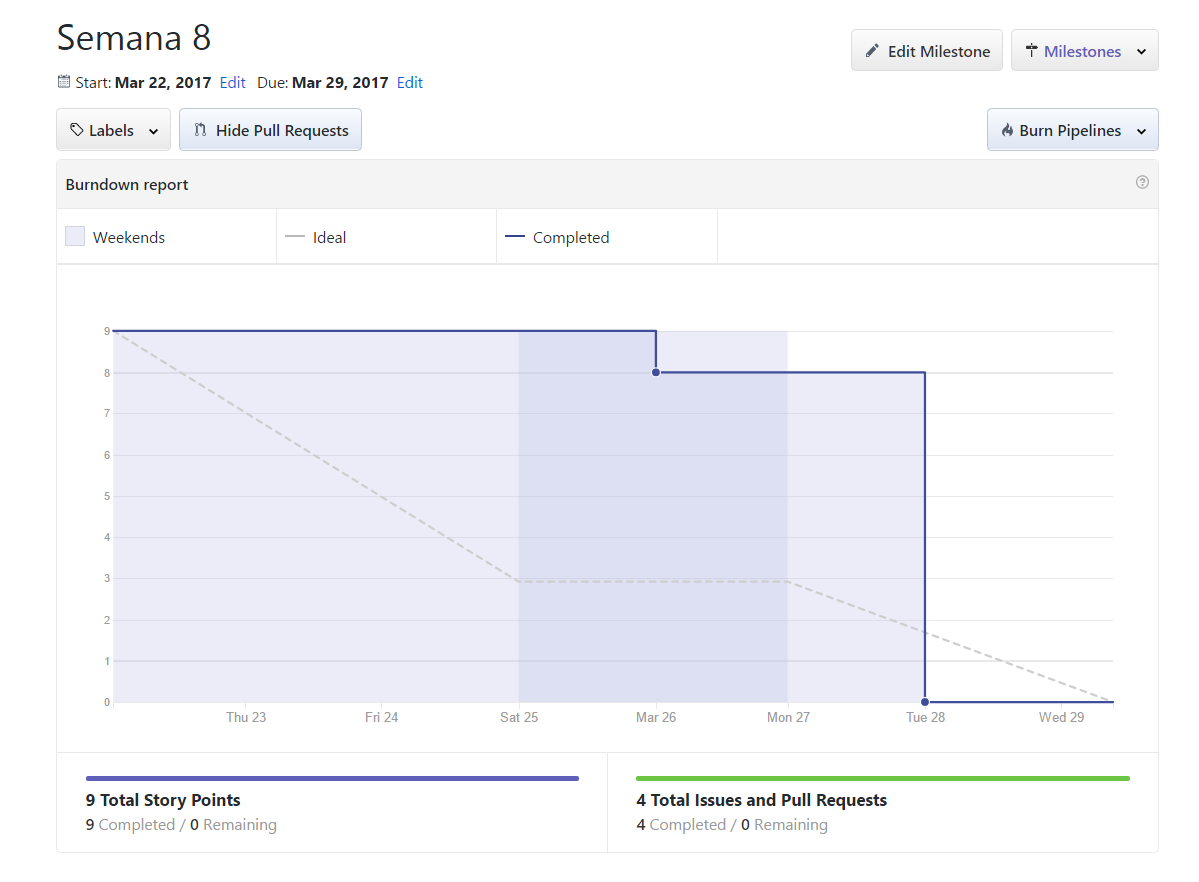
\includegraphics[width=0.99\textwidth]{Semana8}
\caption{Burndown del sprint 7}
\label{fig:A.6}
\end{figure}

Primeramente hay que organizar el código haciéndolo más legible y limpiarlo de comentarios, y pruebas para ver su funcionamiento. Queremos que los resultados queden de una forma similar al Thoth original, para conservar su esencia, usabilidad, y buen diseño. Para ello hacemos uso de Vaadin, una herramienta que se puede utilizar como un <<plugin>> en eclipse y que se integra perfectamente con GWT.

\subsection{Sprint 8 (29/3/2017 - 5/4/2017)}

Al principio de este octavo sprint o 9 semana, estuve pendiente de la respuesta por parte de Vaadin sobre si me podía conceder o no una licencia gratuita, así que me centré en incluir el algoritmo de eliminación de símbolos no terminales, mejorando lo que tenía hasta el momento, que era solo una pequeña interfaz con una funcionalidad que no era la exacta. Por ello me centré en corregirla. Así lo hicimos.

\begin{figure}[h]
\centering
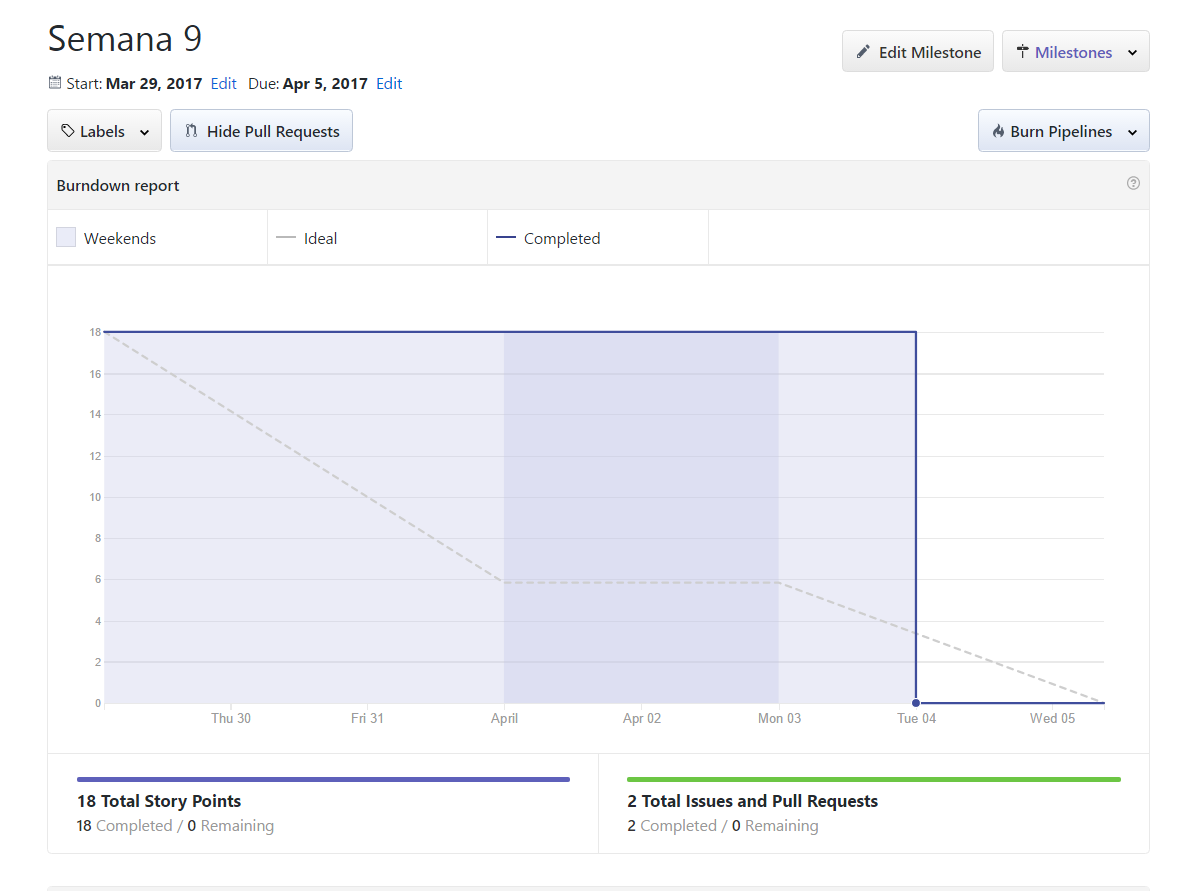
\includegraphics[width=0.99\textwidth]{Semana9}
\caption{Burndown del sprint 8}
\label{fig:A.7}
\end{figure}

Posteriormente llegó la respuesta de Vaadin explicando que no me podía conceder la licencia y que buscase otras opciones dentro de las que ellos mismos me ofrecían. Al principió lo intenté pero resulto que no supe como hacerlo. Lograba hacer un proyecto de Vaadin pero no conseguía incluirlo en el mio propio de GWT.

Así que comencé a hacer la interfaz por mi mismo, con las posibilidades de GWT. Puede verse en el burdown chasr de la ilustración\ref{fig:A.7} como la carga de trabajo se concentra sobre todo en el final.

Las tareas para esa semana fueron: 

\begin{itemize}
\item La inclusión del algoritmo de Eliminacion de símbolos no terminales, de una forma mejorada.
\item Recabar información sobre internacionalización en GWT.
\end{itemize}

Logramos hacer que funcionase el algoritmo como queríamos y estuvimos mejorando el diseño y la funcionalidad de la interfaz de dicho algoritmo.

\subsection{Sprint 9 (05/4/2017 - 19/4/2017)}

Es el sprint más largo hasta la fecha ya que incluye dos semanas de trabajo por coincidir con las vacaciones de Semana Santa. Engloba fundamentalmente el hacer los demás algoritmos, con sus respectivas vistas. El burdown chart del sprint 9 se ilustra en la figura\ref{fig:A.8}.

\begin{itemize}
\item Implementar los algoritmos restantes.
\item Mejorar el código, haciéndolo más comprensible y organizar la parte visual.
\item Hacer la documentación sobre la parte del diseño y sobre las herramientas que tiene la UBU relacionadas con este proyecto.
\end{itemize}

\begin{figure}[h]
\centering
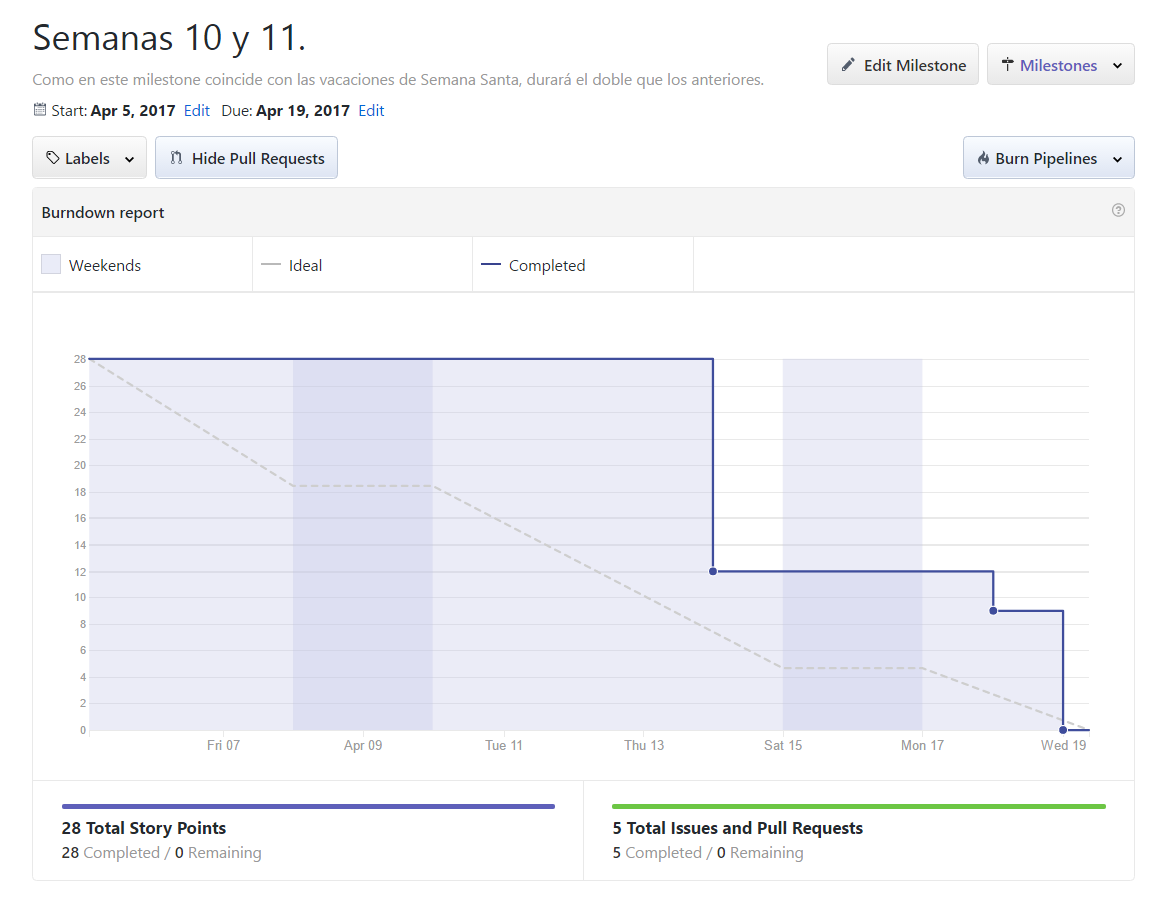
\includegraphics[width=0.99\textwidth]{Semana10-11}
\caption{Burndown del sprint 9}
\label{fig:A.8}
\end{figure}

En estas dos semanas no pude realizar todos los algoritmos como en un principio pretendía porque la parte visual se alejaba de lo que tenia hecho hasta el momento, es decir, necesitaba hacer nuevas vistas que llevaban más tiempo del pensado y no me dio tiempo, pero si que incluí la mayor parte de ellos. Estuvimos estudiando como aplicar el resaltado de las producciones. En el Thoth original utilizaba una librería, java swing, que ya comprobamos anteriormente que no podía ser incluida en GWT en este proyecto así que buscamos otras alternativas como hacer un resaltado a mano con HTML. De momento lo dejamos ahí.

\subsection{Sprint 10 (19/4/2017 - 26/4/2017)}

Una vez pasadas las vacaciones de Semana Santa, el proyecto tiene una forma más madura y podemos ir haciendo añadidos más funcionales a la aplicación. Es por ello que decidimos empezar con la internacionalización, viendo como funcionaba para poder entenderla y una vez entendida incluirla en el proyecto. Además de esto, después de comprobar en la semana pasada que el resaltado lo podíamos hacer con HTML nos dedicamos de lleno a ello. La verdad es que nos llevó muchos quebraderos de cabeza. El porqué no era otra cosa que teníamos que tener en cuenta todo el funcionamiento interno, <<destripar>> que contenía cada variable, como funcionaban cada método de GWT etc. Todo este trabajo nos llevo mucho tiempo, ya que estuvimos todo el sprint a base de prueba y error con los diferentes algoritmos hasta que funcionó en todos de la forma que deseamos. En el burdown chart\ref{fig:A.9} se puede apreciar como no es hasta el final del sprint cuando se cierran los issues.

\begin{figure}[h]
\centering
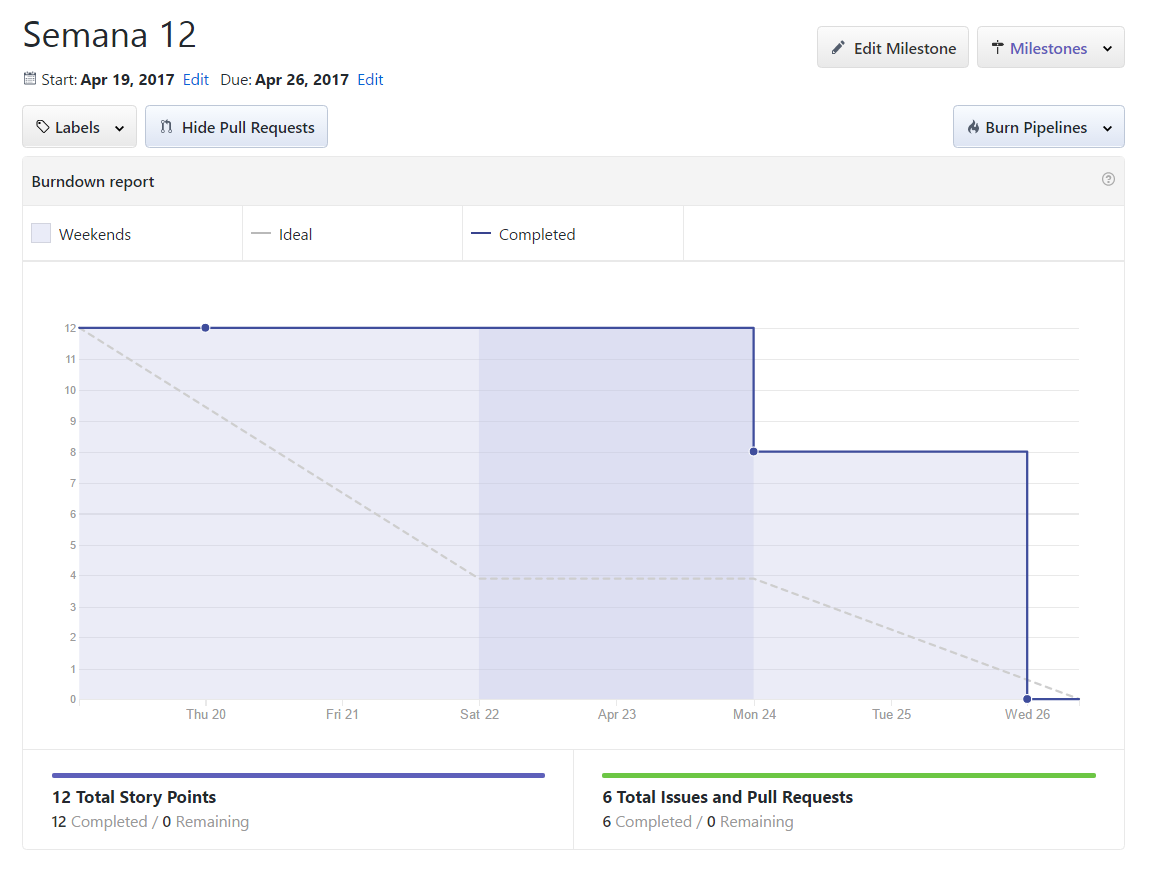
\includegraphics[width=0.99\textwidth]{Semana12}
\caption{Burndown del sprint 10}
\label{fig:A.9}
\end{figure}

Estas fueron las tareas correspondientes a esta semana.

\begin{itemize}
\item Aplicar internacionalización.
\item Cambiar la visualización de los paneles.
\item Resaltado de producciones en los algoritmos con HTML.
\item Incluir los demás algoritmos.
\item Incluir pestañas y elementos de Vaadin.
\end{itemize}

La parte visual, es decir, la inclusión de pestañas en realidad no lo llegamos a aplicar bien, de la forma deseada y se trató en el siguiente sprint. Además los elementos de Vaadin no se pudieron incluir ya que la única forma de añadirlos a un proyecto GWT son con licencias de pago. La visualización de los paneles simplemente fue una recolocación para que quedase más agradable a la vista.


\subsection{Sprint 11 (26/4/2017 - 03/5/2017)}

En la semana 13, seguimos acumulando un pequeño <<bug>> en el resaltado de las producciones, y es que la interpretación de las comillas dobles <<``''>> no las interpretaba como nosotros queríamos y por ello no hacía un buen borrado del resaltado, manteniéndose en cada paso. La solución fue simplemente sustituirlas por las comillas dobles de java <</``>>. Pero las dos grandes tareas de esta semana consistieron en aplicar el algoritmos FirstFollow y un TabLayoutPanel para hacer un panel con pestañas como los que se ven en los navegadores web.

Las tareas quedaron asi.

\begin{itemize}
\item Solucionar bug en el resaltado.
\item Implementar algoritmo FirstFollow.
\item Incluir TabLayoutPanel para hacer diferentes pestañas.
\end{itemize}

El algoritmo FirstFollow fue fácil hasta el momento de mostrar los resultados en las tablas. Resulta que al tratar de imprimir los resultados de tipo Object pasándolos como un <<string>> no los reconocía bien. Este tipo de errores no son fáciles de detectar en GWT, ya que la forma para verlos claramente es imprimiendo los valores por pantalla y tratando de analizarlos, en que formato están etc. Al final descubrimos que el problema era al tratar de pasara al formato string valores que GWT interpretaba como <<undefined>> y que no eran más que valores en blanco, espacios en blanco dentro de la tabla. Se puden ver mas detalles en la figura\ref{fig:A.10}.

\begin{figure}[h]
\centering
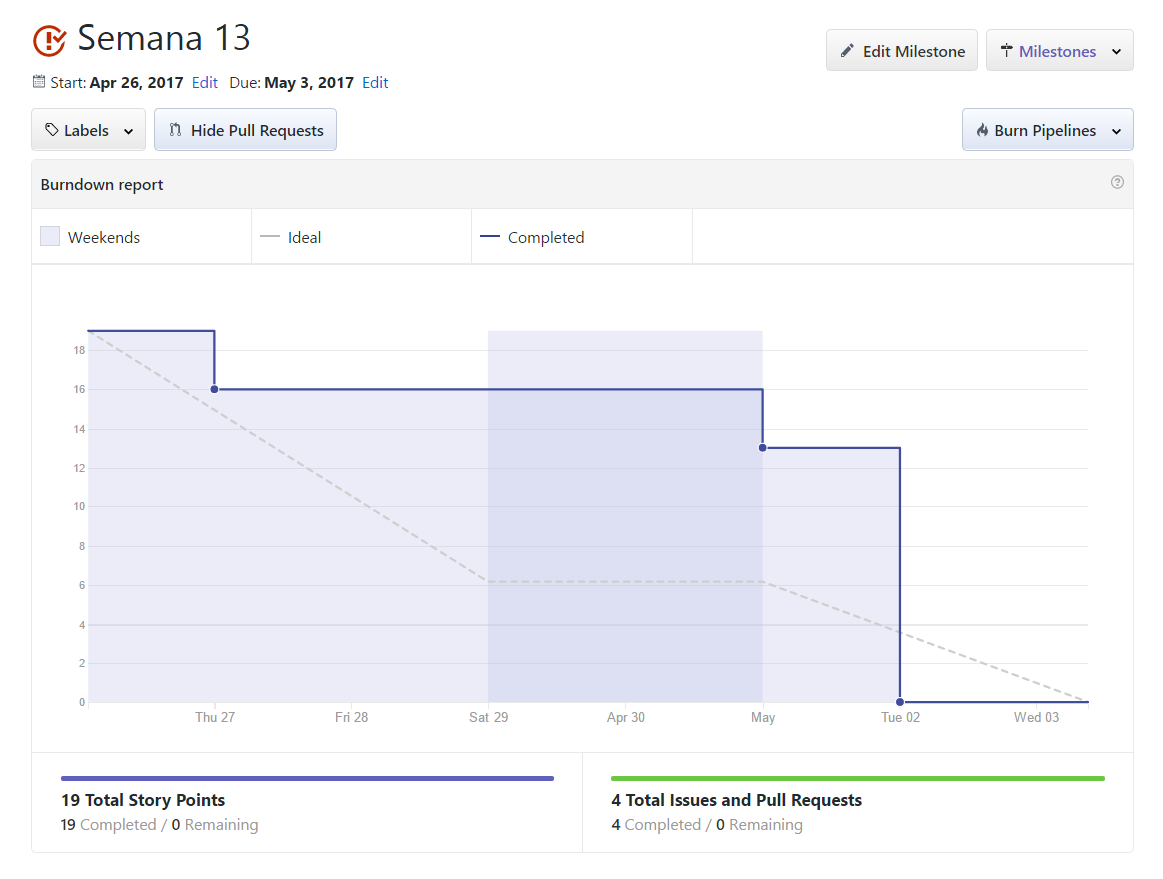
\includegraphics[width=0.99\textwidth]{Semana13}
\caption{Burndown del sprint 11}
\label{fig:A.10}
\end{figure}

El otro gran quebradero de cabeza fue el tratar de incluir pestañas en la aplicación. No es nada fácil añadir una pestaña con una nueva vista sin que esta remplace otra, se superponga o cualquier otra cosa. A día de hoy no sabemos bien el porqué de esto al cien por cien. Lo que si es cierto es que no es completamente necesaria y se puede hacer un reemplazamiento de otras vistas.

\subsection{Sprint 12 (03/5/2017 - 10/5/2017)}

Entrado en el mes de mayo, la recta final del proyecto, y con una aplicación base ya consolidada, por denominarlo así, nos dedicamos sobre todo ha hacer mejoras en cuanto a temas visuales y funcionales. Además de esto el objetivo en este mes es hacer un registro e inicio de sesión de los usuarios para así tener un control detallado del uso.
Con todo esto por un lado, también era hora de dedicarle un porcentaje de tiempo mayor a documentar el proyecto. Véase la ilustración\ref{fig:A.11}.

\begin{figure}[h]
\centering
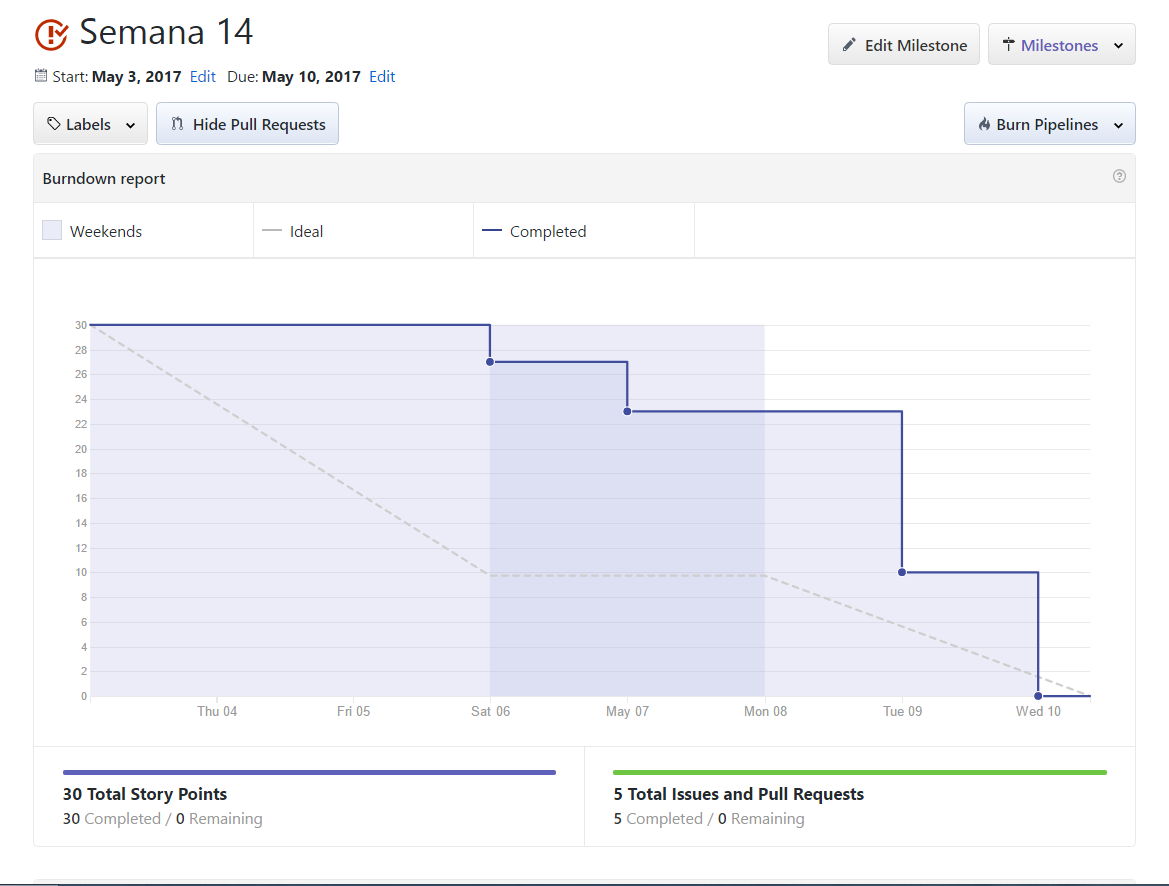
\includegraphics[width=0.99\textwidth]{Semana14}
\caption{Burndown del sprint 12}
\label{fig:A.11}
\end{figure}

Para esta semana determinamos que las tareas quedaría de esta manera:

\begin{itemize}
\item Comenzar a estudiar y probar el inicio de sesión.
\item Actualizar la documentación.
\item Mejoras en la interfaz (botones, colores y formas).
\item Añadir un control de errores más elaborado y hacer la aplicación más robusta.
\item Cambiar la funcionalidad de los botones en los algoritmos.
\end{itemize}

La tarea de cambiar la funcionalidad de los botones en los algoritmos hace referencia a que regrese o vaya a una vista u otra dependiendo del botón pulsado o de las acciones asociadas a ello.
Las mejoras visuales son hechas a mano, como ya he comentado anteriormente, y es por ello que es un trabajo largo, en el que hay que estar compilando continuamente para ver los efectos resultantes, que no siempre son los esperados.
El inicio de sesión acabó en un ejemplo con varios errores y algo chapucero que sirvió para comprender el funcionamiento por lo que no se mejoró nada en la aplicación.

\subsection{Sprint 13 (10/5/2017 - 17/5/2017)}

Llegados a este punto comenzamos a <<pulir>> lo que tenemos añadiendo estilos con CSS y mejorando pequeños aspectos como es el caso de la vista de los algoritmos. Al resaltar los pasos en un algoritmo, tuvimos la <<necesidad>> de utilizar un RichTextArea para poder manejar el código HTML y poder así subrayarlo. Más tarde nos dimos cuenta de que este tipo de área no se puede inhabilitar para que no se editable y esto se trata de un bug de GWT, la función está pero no hace nada. Otros usuarios también se quejaron de ello. Así que decidimos meterlo todo dentro de un panel como texto normal en HTML, que al fin y al cabo era lo que ya habíamos hecho. El burdown chart se ilustra en la figura \ref{fig:A.12}.

Los issues quedaron definidos así:
\begin{itemize}
\item Cambiar las interfaces de las gramáticas.
\item Incluir nuevos estilos.
\item Documentar aspectos como la introducción y los conceptos teóricos.
\item Añadir una nueva clase para hacer la internacionalización.
\item Solucionar un bug que surgió sobre la vista de los algoritmos.
\item Aplicar un pequeño ejemplo de inicio de sesión.
\end{itemize}

\begin{figure}[h]
\centering
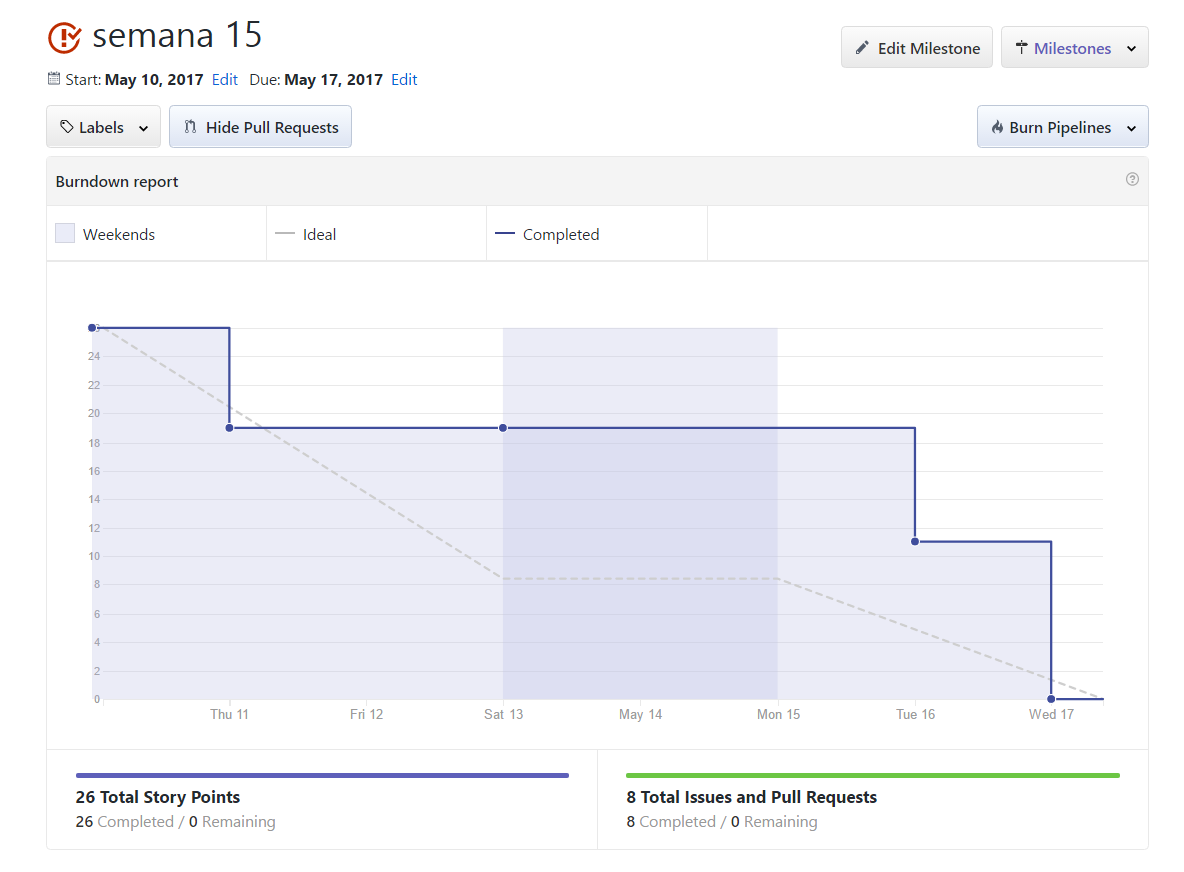
\includegraphics[width=0.99\textwidth]{Semana15}
\caption{Burndown del sprint 13}
\label{fig:A.12}
\end{figure}

Se pudo hacer un ejemplo en un proyecto a parte para hacer un simple inicio de sesión sin base de datos. Para lograr el inicio se hizo por medio de cookies. El objetivo siguiente sería poder aplicar esto a nuestro proyecto pero con una pequeña base de datos en la cual se registraban los usuarios y luego hacían inicio de sesión. También añadimos clases para que encapsularan la internacionalización y poder lanzar mensajes de aviso.

\subsection{Sprint 14 (17/5/2017 - 24/5/2017)}

En el sprint 14, es decir la decimosexta semana, se centraron los esfuerzos sobre todo en hacer un registro e inicio de sesión de usuarios. La idea inicial era la de guardar información de nombre, apellido, un correo que sirviera de identificador único y una contraseña. Para ello se creó una pequeña base de datos, casi podríamos hablar de repositorio. Una vez registrados esos datos el usuario tendría un perfil creado y podría acceder a la aplicación.

Las tareas se centraron en documentar y hacer el registro y sesión de usuarios:
\begin{itemize}
\item Añadir un login o inicio se sesión.
\item Corregir aspectos de la documentación.
\item Incluir alguna mejora en el menú principal.
\end{itemize}

\begin{figure}[h]
\centering
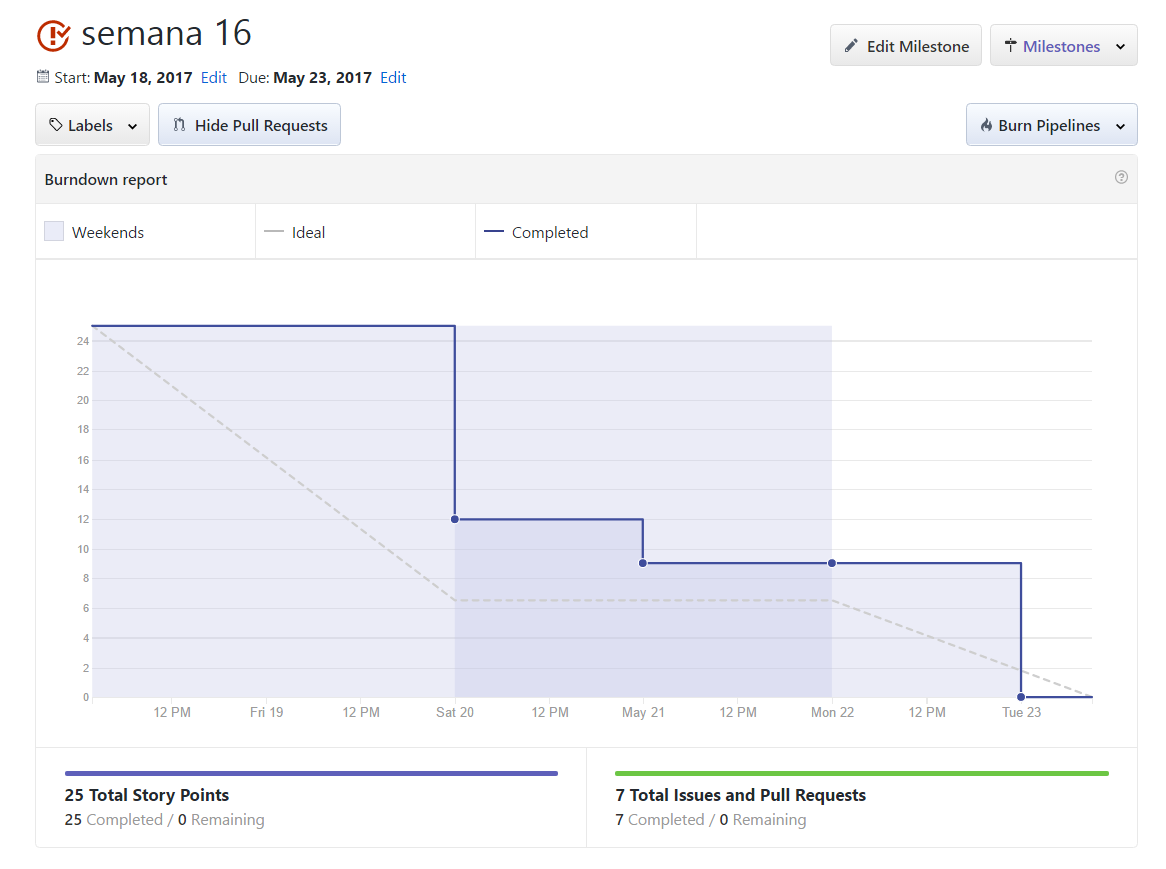
\includegraphics[width=0.99\textwidth]{Semana16}
\caption{Burndown del sprint 14}
\label{fig:A.13}
\end{figure}

Además de esto, surgió un bug o pequeño error con los estilos <<css>>. Y es que al crear varios módulos para realizar varias vistas en la aplicación los estilos, que son propios de cada módulo, se solapaban y se mezclaban mostrando en un módulo el estilo del otro y viceversa. El error no tenía mucha complicación y se pudo solucionar sin problema. Puede verse el burdown en la ilustración\ref{fig:A.13}.
El registro e inicio de sesión me llevo tiempo, dos sprints el hacer lo básico y otros dos <<pulirlo>> ya que los conceptos en cuanto a carga de módulos, y comunicación RPC eran en parte nuevos. Lo demás fue principalmente documentación, mejorarla y continuar con lo anterior.

\subsection{Sprint 15 (24/5/2017 - 31/5/2017)}

Ya en la semana 17, una vez que tenemos la base de datos haciendo el registro de usuarios nos metemos con la codificación de las contraseñas. Consiste en crear una clave secreta generada por medio de una función con la que ciframos la contraseña para mantener la privacidad de los datos de los usuarios registrados. 

Los <<issues>> para este sprint son:
\begin{itemize}
\item Cifrado de contraseñas.
\item Registro de más información.
\item Mejorar el aspecto del <<login>>
\end{itemize}

El registro de más información consiste en añadir a la base de datos la fecha de registro de un usuario o la última vez que inició sesión en la aplicación. La resolución de los issues queda reflejada en la siguiente gráfica ilustrada en la figura\ref{fig:A.14}.

\begin{figure}[h]
\centering
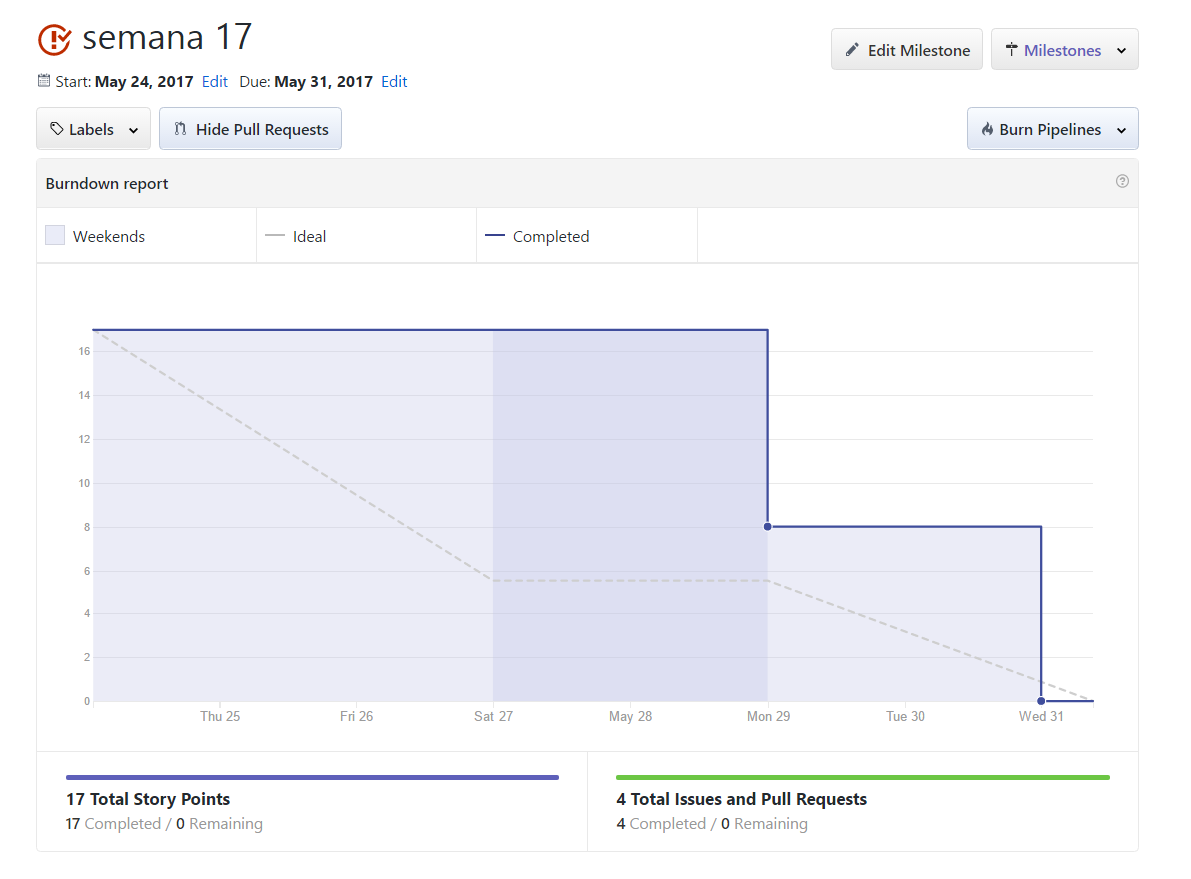
\includegraphics[width=0.99\textwidth]{Semana17}
\caption{Burndown del sprint 15}
\label{fig:A.14}
\end{figure}

Además de esto, añadimos algunos estilos a las vistas de inicio y registro de sesión aunque posteriormente lo volveremos a modificar, hasta estar a gusto con el diseño.

\subsection{Sprint 16 (31/5/2017 - 7/6/2017)}

En el sprint número dieciséis tratamos de pulir un poco lo que tenemos. Para ello limpiamos el código refactorizando y dando nombres a las variables con un sentido más específico, comentando un poco el código y eliminando aquello que no nos es útil. Arreglamos algún <<bug>> que aparece en el renombrado de nodos por ejemplo.


Para esta semana las tareas son las siguientes.
\begin{itemize}
\item Cifrado de contraseñas.
\item Validación de e-mail.
\item Añadir tratamiento de errores en el login.
\item Refactorizar el código.
\end{itemize}

Seguimos con el cifrado de contraseñas porque decidimos mejorarlo y dejarlo más claro y con más posibilidades, dependiendo de las iteraciones y de las variables podemos crear un nivel de cifrado más simple o más complejo. 

A su vez comprobamos que la dirección de correo introducida cumpla con la <<plantilla>> de una dirección real. Consiste en hacer una comprobación por medio de HTML y una función en Java bastante simple. El burdown queda de esta manera\ref{fig:A.15}.

\begin{figure}[h]
\centering
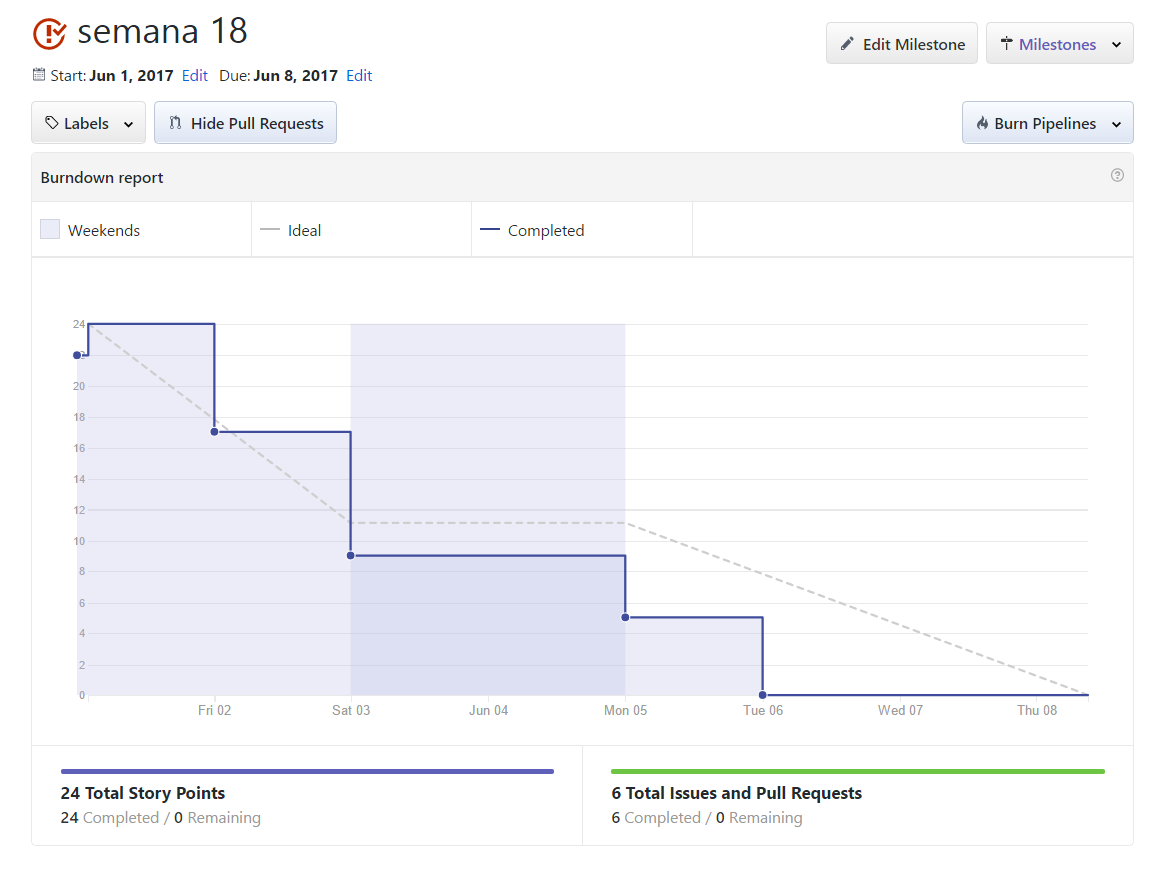
\includegraphics[width=0.99\textwidth]{Semana18}
\caption{Burndown del sprint 16}
\label{fig:A.15}
\end{figure}

Además de esto añadimos imágenes de fondo, el escudo de la universidad de Burgos en el inicio de sesión y registro de usuarios. Esta semana tiene un poco menos de carga de trabajo porque coincide con fechas de exámenes.


\section{Estudio de viabilidad}

En este apartado se realiza un estudio de viabilidad del proyecto que consiste utilizar la
técnica del análisis conste/beneficio.Con ello se obtiene una valoración de la justificación económica del proyecto.

El estudio de la viabilidad se divide en la
viabilidad económica y la viabilidad legal.
Para el estudio de viabilidad económica se supone que el proyecto ha sido realizado
dentro del ámbito empresarial. Quiere decir que se considera que los alumnos han recibido un sueldo por en base a la legislación por realizarlo.


\subsection{Viabilidad económica}

Para analizar la viabilidad económica, hay que tener en cuenta los constes de personal y los costes de material.

\subsubsection{Costes de personal}

Se cuenta como coste personal el trabajo del alumno, considerado como un programador junior. La duración del trabajo a sido de 5 meses, unos con más carga de trabajo que otros. Estimo unas 460 horas de trabajo y analizando un poco los sueldo de los programadores junior en Java que ronda los 9 euros la hora, el resultado es el siguiente.

\[ 460h * 9\textrm{\euro/h} = 4140\textrm{\euro}\]

A esto, debemos sumarle la Seguridad Social y otros impuestos que se deben pagar por empleado. En la actualidad, los costes a cargo de una empresa son los siguientes:

\begin{itemize}
\item Contingencias Comunes: 23,60\%
\item Desempleo de Tipo General: 5,50\%
\item Fondo de Garantía Social: 0,2\%
\item Formación profesional: 0,6\%
\item \textbf{Total:} 29.9\%
\end{itemize}

Que esto equivale a un gasto por un trabajador de: 
\[ 4140\textrm{\euro} * 0,299 = 1237,86\textrm{\euro}\]
\subsubsection{Costes de material}

Como costes materiales se tienen en cuenta el software y el hardware. El software es todo ello gratuito y no necesita ninguna licencia bajo pago. En cuanto al hardware tendremos en cuenta el equipo en el cual se ha desarrollado. Se trata de un computador con un valor de 980\euro, que teniendo en cuenta su amortización media de unos 5 años de uso, el cálculo sería el siguiente. 
\[ \frac{980\textrm{\euro}}{12\textrm{meses} * 5 \textrm{periodos}} *5\textrm{meses de uso} = 81,66\textrm{\euro}\]
 
Por lo tanto los costes totales quedaría reflejados en la siguiente tabla \ref{tab:costes}.

\begin{table}[]
\centering
\rowcolors {2}{gray!35}{}
%\resizebox{0.5\textwidth}{!}{
\begin{tabular}{p{4cm} p{2cm}}
\toprule
Costes & Importe \\ \midrule
Personal         & 4140 \euro{}   \\ 
Seguridad Social & 1237,86\euro{} \\ 
Material         & 81,66\euro{}   \\ 
\textbf{Total}   & \textbf{5459,52\euro{}} \\ \bottomrule
\caption{Tabla de los costes totales}
\label{tab:costes}

\end{tabular}
%}
\end{table}

\subsection{Viabilidad legal}

En el marco de la viabilidad legal, se debe considerar las licencias de los programas y librerías utilizados para la realización de la aplicación.

Para el desarrollo del proyecto se ha hecho uso del framework GWT, que cuenta con la Licencia Apache 2.0, que es una licencia software libre permisiva compatible con GPL y aprobada por la Open Source Initiative. Esto se traduce en que el software producido bajo los términos de esta licencia otorga a usuario la utilización del software para cualquier propósito de modificación o distribución.

Las librerías que se emplean también son gratuitas y de código abierto.
